
\documentclass[12pt]{article}
\usepackage[english]{babel}
\usepackage[utf8x]{inputenc}
\usepackage{amsmath}
\usepackage{graphicx}
\usepackage[colorinlistoftodos]{todonotes}
\usepackage[margin=1in]{geometry}
\usepackage{listings}
\usepackage{color}
\renewcommand\lstlistingname{Quelltext} % Change language of section name

\lstset{ % General setup for the package
	language=Perl,
	basicstyle=\small\sffamily,
	numbers=left,
 	numberstyle=\tiny,
	frame=tb,
	tabsize=4,
	columns=fixed,
	showstringspaces=false,
	showtabs=false,
	keepspaces,
	commentstyle=\color{red},
	keywordstyle=\color{blue}
}

\begin{document}
\begin{titlepage}

\newcommand{\HRule}{\rule{\linewidth}{0.6mm}} % Defines a new command for the horizontal line, Thickness can be changed

\center % Center everything on the page
 
%----------------------------------------------------------------------------------------
%	HEADING
%----------------------------------------------------------------------------------------

\textsc{\huge Telecommunication Software Lab}\\[1.5cm] % software lab course name
\textsc{\Large ELP 718}\\[0.5cm] % Course Code
%----------------------------------------------------------------------------------------
%	Assignment Number
%----------------------------------------------------------------------------------------

\HRule \\[0.4cm]
{ \large \textit {Assignment 6}}\\[0.4cm] % Title of your document
\HRule \\[1.5cm]
 
%----------------------------------------------------------------------------------------
%	Personal Details
%----------------------------------------------------------------------------------------

\begin{minipage}{0.4\textwidth}
\begin{flushleft} \Large
\emph{Name:}\\
\textbf{Chanchal Kumar}%My Name
\end{flushleft}
\end{minipage}
~
\begin{minipage}{0.4\textwidth}
\begin{flushright} \Large
\emph{Entry Number:} \\
\textbf{2017JTM2018} % Entry Number
\end{flushright}
\end{minipage}\\[2cm]


%----------------------------------------------------------------------------------------
%	DATE SECTION
%----------------------------------------------------------------------------------------

{\large \today}\\[4cm] % Date

%----------------------------------------------------------------------------------------
%	LOGO
%----------------------------------------------------------------------------------------


\includegraphics[scale=.5]{logo.png}\\[1cm] % IIT Delhi Logo
\LARGE{INDIAN INSTITUTE OF TECHNOLOGY}\\
{\Large{NEW DELHI}}\\
\HRule
%----------------------------------------------------------------------------------------

\vfill % Fill the rest of the page with whitespace

\end{titlepage}

%----------------------------------------------------------------------------------------
%Contents
%----------------------------------------------------------------------------------------
\newpage %new page

\tableofcontents

\newpage

\section{Problem Statement 1: }
You have to do parity check and bit stuffing to make a frame in this problem.
Parity Check
The simplest way of error detection is to append a single bit , called a parity check, to a string of data bits. This parity check bit has the value 1 if number of 1’s in the bit string is even and has the value 0 otherwise, i.e., Odd Parity Check.

Bit Oriented Framing
Data Link Layer needs to pack bits into frames, so that each frame is distinguishable from another. Frames can be fixed or variable size. In variable size framing, we define end of frame using bit oriented approach. It uses a special string of bits, called a flag for both idle fill and to indicate the beginning and the ending of frames.
The string 0101 is used as the bit string or flag to indicate the end of the frame. The bit stuffing rule is to insert a 0 after each appearance of 010 in the original data. In addition, if the frame ends in 01, a 0 would be stuffed after the 1st 0 in the actual terminating string 0101.




\subsection{Assumptions}
Parity check is following odd parity check.




\subsection{Program Structure}
\begin{itemize}


\item In first line of the program You have to enter Enter binary bit data which has to be transmitted.

\item Program will Print binary bit data with parity bit.

\item Then Print the modified string received at the other end.

\end{itemize}
\subsection{Graphical Structure of Code}

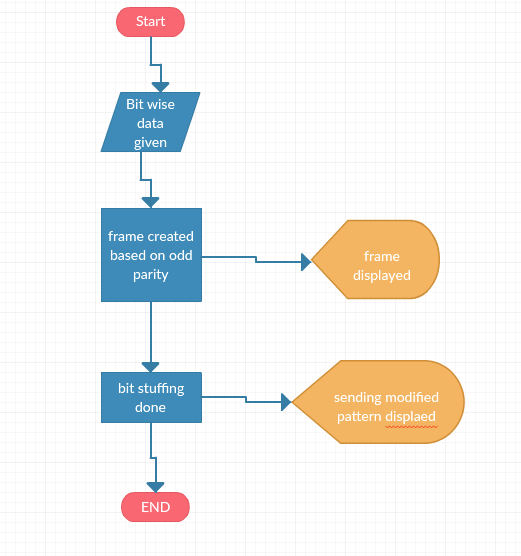
\includegraphics[width=0.9\textwidth]{flowpy1.png}



%\subsection{Theoretical structure of code}
 
% \includegraphics[width=0.5\textwidth]{theory.png}\\



\subsection{Algorithm and Implementation}

For parity check i have counted number of 1 , if it is even frame is concatenated with 1 otherwise with 0.

\subsection{Input and Output format}

\textbf{Input format:}


Enter binary bit data which has to be transmitted.



\textbf{Output format:}

Print binary bit data with parity bit.
Print the modified string received at the other end.
	



\subsection{Test cases}
\begin{itemize}


\item Case 1:
input 1001011
Frame with parity bit = 10010111
Modified string = 1001001110101

\item Case 2:
Input 10110101101100
Frame with parity bit = 101101011011001
Modified string received= 101101001100100101


\end{itemize}


\subsection{Difficulties/Issues faced}
difficulty faced in bit stuffing while consecutive 010101 pattern arrives.
in this it will bit stuff as 0100101 as program is searching and replacing for 010.
\subsection{Screenshots}
Test Cases Output Screenshots:




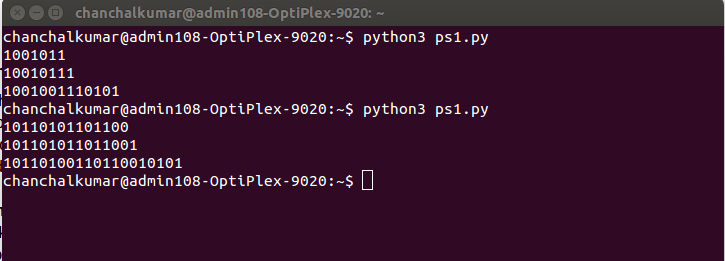
\includegraphics[width=0.8\textwidth]{screenpy1.png}\\


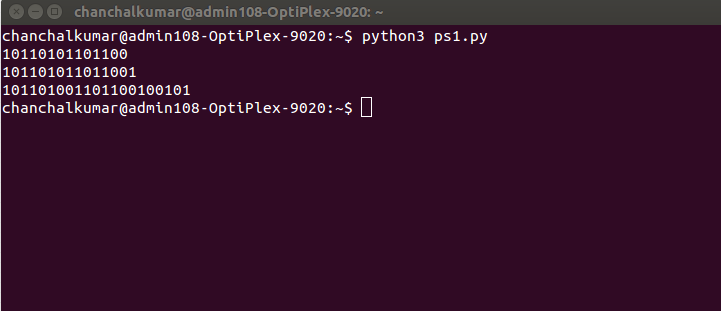
\includegraphics[width=0.8\textwidth]{screenpy2.png}\\


%\includegraphics[width=0.8\textwidth]{screen3.png}\\


%\includegraphics[width=0.8\textwidth]{screen4.png}\\

\newpage


\section{Problem Statement 2: }
3X3 Numeric Tic-Tac-Toe (Use numbers 1 to 9 instead of X’s and O’s)
One player plays with the odd numbers (1, 3, 5, 7, 9) and other player plays with the even numbers (2,4,6,8). All numbers can be used only once. The player who puts down 15 points in a line wins (sum of 3 numbers). Always Player with odd numbers start the game. Once a line contains two numbers whose sum is 15 or greater, there is no way to complete that line, although filling in the remaining cell might be necessary to complete a different line.
Note – Line can be horizontal, vertical or diagonal

Constraints:
\begin{itemize}
\item position between 1 and 9 

\item number between 1 and 9 

\item sum between 1 and 15
\end{itemize}





\subsection{Assumptions}


\subsection{Program Structure}
\begin{itemize}


\item Welcome priented

\item Position and number entered from user
\item tic tac tow data showed

\item continue till wining.

\end{itemize}
\subsection{Graphical Structure of Code}

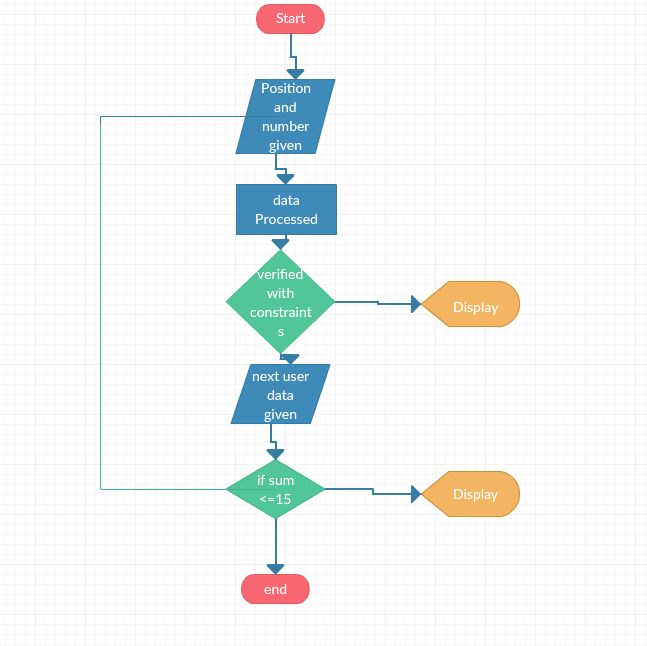
\includegraphics[width=0.9\textwidth]{flowpy2.png}



%\subsection{Theoretical structure of code}
 
% \includegraphics[width=0.5\textwidth]{theory.png}\\



\subsection{Algorithm and Implementation}



\subsection{Input and Output format}
Terminal:
\begin{itemize}
\item Print ‘Welcome to the Game!’.	
\item Print whether it is Player 1’s or Player 2’s chance.
\item Get the position and number to be entered from user.
\item Show 	tic tac toe with data.
\item Continue till the game gets draw or some player wins and show result.
\item Ask user whether to continue for next game or exit.

sample output: 
Welcome to the Game!
Player 1’s chance
Enter the position and number to be entered: 5,3

\end{itemize}

\subsection{Test cases}
\begin{itemize}


\item Case1:
Enter the position and number to be entered: 5,3



\end{itemize}


\subsection{Difficulties/Issues faced}
difficulty in running program.
\subsection{Screenshots}
Test Cases Output Screen-shots:



%\includegraphics[width=0.7\textwidth]{screen6.png}\\



%\includegraphics[width=0.7\textwidth]{screen7.png}\\


\newpage


\begin{thebibliography}{9}
\bibitem{tutorial} 
 www.tutorialspoint.com/python
 
\bibitem{studytonight} 

https://www.programiz.com/python-programming
 
\
bibitem{geeksweb} 
https://readwrite.com/2013/09/30/understanding-github-a-journey-for-beginners-part-1/

\bibitem{server} 
http://www.linuxhowtos.org/

\bibitem{server} 
https://inventwithpython.com/chapter10.html
\end{thebibliography}
 
\newpage
\subsection* {Annexture}
Source code for PS1
\begin{lstlisting}
###### Assignment 1 parity check and framing .py file ###########

####### write your code here ##########

def parity(x):        # function for parity bit
	z=x.count('1')
	if z%2==1:
		return 0
	else:
		return 1

x= input()
x=str(x)
z=parity(x)
z=str(z)
frame=(x+z)
print(frame)    #frame after parity bit addition

m=frame.replace('010','0100')  #bit stuffing
u=m[-2:]   #for accessing last 2 character
d='01'
d=str(d)
if u == d:
	m=m+'0'

final= m+'0101'    #modified string received at other end  
print(final)

	


###### this is the second .py file ###########

####### write your code here ##########


#  board
board= [0,1,2,
        3,4,5,
        6,7,8]

def disp():
	print board[0],'|',board[1],"|",board[2]
	print "----------"
	print board[3],'|',board[4],"|",board[5]
	print "----------"
	print board[6],'|',board[7],"|",board[8]

def isWinner(bo, Player1):
    # Given a board and a player's letter, this function returns True if that player has won.
    # We use bo instead of board and le instead of letter so we don't have to type as much.
    return ((bo[7] + bo[8] + bo[9]) >=15) or # across the top
    ((bo[4]+ bo[5] + bo[6]) >=15) or # across the middle
    ((bo[1] + bo[2] + bo[3]) >=15 ) or # across the bottom
    ((bo[7] +bo[4]+bo[1]) =>15) or # down the left side
    ((bo[8] + bo[5] + bo[2] )=>15) or # down the middle
    ((bo[9] + bo[6] + bo[3] )=>15) or # down the right side
    ((bo[7] +  bo[5] + bo[3] )=>15) or # diagonal
    ((bo[9] + bo[5] + bo[1] )=>15)) # diagonal
def playAgain():
    # This function returns True if the player wants to play again, otherwise it returns False.
    print('Do you want to play again? (yes or no)')
    return input().lower().startswith('y')

while True:
	print "Welcome to the Game"
	position= 

\end{lstlisting}



source code for ps2
\begin{lstlisting}
###### this is the second .py file ###########

####### write your code here ##########


#  board
board= [0,1,2,
        3,4,5,
        6,7,8]

def disp():
	print board[0],'|',board[1],"|",board[2]
	print "----------"
	print board[3],'|',board[4],"|",board[5]
	print "----------"
	print board[6],'|',board[7],"|",board[8]

def isWinner(bo, Player1):
    # Given a board and a player's letter, this function returns True if that player has won.
    # We use bo instead of board and le instead of letter so we don't have to type as much.
    return ((bo[7] + bo[8] + bo[9]) >=15) or # across the top
    ((bo[4]+ bo[5] + bo[6]) >=15) or # across the middle
    ((bo[1] + bo[2] + bo[3]) >=15 ) or # across the bottom
    ((bo[7] +bo[4]+bo[1]) =>15) or # down the left side
    ((bo[8] + bo[5] + bo[2] )=>15) or # down the middle
    ((bo[9] + bo[6] + bo[3] )=>15) or # down the right side
    ((bo[7] +  bo[5] + bo[3] )=>15) or # diagonal
    ((bo[9] + bo[5] + bo[1] )=>15)) # diagonal
def playAgain():
    # This function returns True if the player wants to play again, otherwise it returns False.
    print('Do you want to play again? (yes or no)')
    return input().lower().startswith('y')

def getBoardCopy(board):
    # Make a duplicate of the board list and return it the duplicate.
    dupeBoard = []

    for i in board:
        dupeBoard.append(i)

    return dupeBoard

def isSpaceFree(board, move):
    # Return true if the passed move is free on the passed board.
    return board[move] == ' '

def getPlayerMove(board):
    # Let the player type in his move.
    move = ' '
    while move not in '1 2 3 4 5 6 7 8 9'.split() or not isSpaceFree(board, int(move)):
        print('What is your next move? (1-9)')
        move = input()
    return int(move)

def chooseRandomMoveFromList(board, movesList):
    # Returns a valid move from the passed list on the passed board.
    # Returns None if there is no valid move.
    possibleMoves = []
    for i in movesList:
        if isSpaceFree(board, i):
            possibleMoves.append(i)

    if len(possibleMoves) != 0:
        return random.choice(possibleMoves)
    else:
        return None
while True:
	print "Welcome to the Game"
	position= 
\end{lstlisting}


\end{document}
